\documentclass[runningheads]{llncs}

\usepackage[T1]{fontenc}
% \usepackage[dvipdfmx]{graphicx}
\usepackage{graphicx}
\usepackage{amsmath}
\usepackage{algorithm}
\usepackage{algpseudocode}

\begin{document}

\title{
    Generative Model of Suitable Meme Sentences for Images using AutoEncoder
    % \thanks{This work is supported by the Japan Society Promotion of Science(JSPS), KAKENHI(20K11979).}
}

\author{
    Ryo Yamatomi    \orcidID{0000-0003-0524-2888} \and \\
    Shahrzad Mahboubi   \orcidID{0000-0002-9577-3721} \and \\
    Hiroshi Ninomiya    \orcidID{0000-0003-3418-3178}
}

\authorrunning{R. Yamatomi et al.}
\titlerunning{GUMI-AE}

\institute{
    Shonan Institute of Technology(SIT), \\ 
    1-1-25 Tsujido-nishikaigan, Fujisawa, Kanagawa, 251-8511, Japan \\
    \email{\{23T2003@sit, shaa@info, ninomiya@info\}.shonan-it.ac.jp}\\
    % \url{https://www.shonan-it.ac.jp}
}

\maketitle

\begin{abstract}
This paper proposes a new image caption generative model for $ Meme $s called GUMI-AE. Meme denotes a humorous short sentence suitable for the given image in this paper. An Image caption generative model usually consists of an image encoder and a sentence decoder. Furthermore, most conventional models use a pre-trained neural network model for the image encoder, e.g., ResNet152 trained using ImageNet. However, pre-trained ResNet152 may not be effective as an encoder for extracting features from arbitrary images. Because the training samples for the meme generative model can be obtained from the website "Bokete" (in Japanese) which is a website that provides a system for people to post images and humorous short sentences associated with these images. Images posted on Bokete include a wide variety of images such as illustrations and text-only images which may be outside of the training images of ImageNet. This paper proposes an image caption generative model incorporating AutoEncoder(AE) as the image encoder. AE can be trained with the training samples obtained from Bokete without the image annotation. This enables the proposed method to generate short sentences with humor for memes. Finally, the proposed model is compared with the conventional one, and the evaluation of the proposed GUMI-AE will be discussed.

\keywords{
    Image caption generative model \and 
    Meme \and 
    Neural Networks \and 
    AutoEncoder.
}
\end{abstract}

\section{Introduction}

\begin{figure}[!t]
    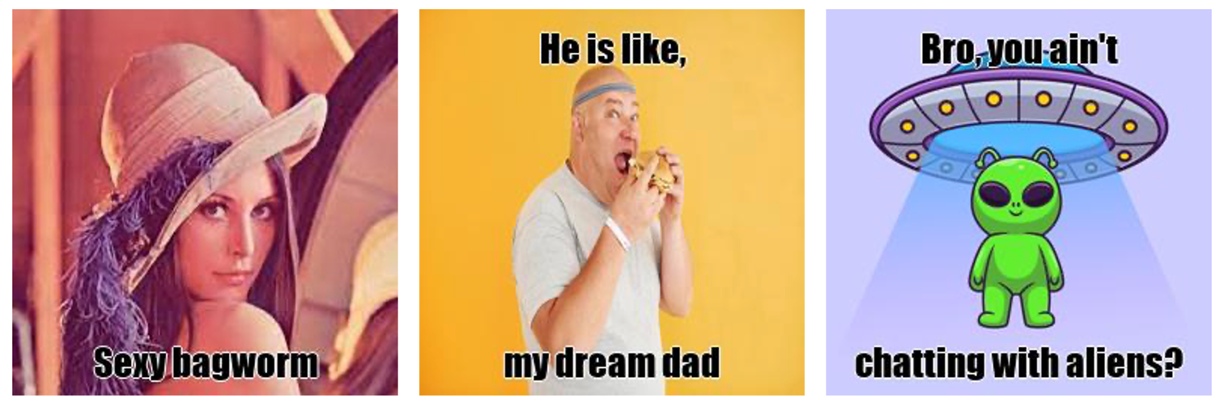
\includegraphics[width=\textwidth]{MEME_example.png}
    \caption{Some meme examples generated by proposed GUMI-AE.} \label{fig_meme_example}
\end{figure}

~~ In recent years, due to the rapid development of a generative model, it has been applied in various fields, and a wide variety of studies have been conducted. Some significant studies on generative models include Generative Adversarial Network \cite{ref_GAN}, Generative Pre-trained Transformer (GPT) \cite{ref_ChatGPT} and Meme generator using the image caption generative model \cite{ref_Show_And_Tell} is attracted in this field.
A meme is one of the cybercultures spreading and attracting attention worldwide, especially on social networking services(SNS), for entertainment and communication in a society where the internet has become very widespread \cite{ref_meme}. They are images and videos with jokes or humorous short sentences and are meme is usually created by pasting short sentences onto an image or video. Some meme examples for images are shown in figure \ref{fig_meme_example}. These memes are generated by the proposed GUMI-AE. 
The data flow of the image caption generative model is shown in figure \ref{fig_image_caption_example}. As figure \ref{fig_image_caption_example} shows, an image caption generative model usually consists of an image encoder and a sentence decoder. In the image caption generative model, an image is given as input to the image encoder and converted into a feature represented by a vector. The feature is input to a sentence decoder. The sentence decoder uses its feature vector to generate words in time series to construct a sentence. In many research and implementation, a pre-trained model, e.g. ResNet152 \cite{ref_ResNet152} or Inception-v3 \cite{ref_Inception_v3}, trained using ImageNet \cite{ref_ImageNet}, is used as the image encoder \cite{ref_Show_And_Tell,ref_Dank_Learning,ref_NJM}. ImageNet is a large dataset consisting of photographs of animals, vehicles, etc. Models pre-trained on this data are expected to have high feature extraction capability for common images.
As an approach to generate memes by AI, English-based \cite{ref_Dank_Learning} and Japanese-based Neural Joking Machine (NJM) \cite{ref_NJM} have been proposed. In \cite{ref_Dank_Learning}, to generate memes for images, Inception-V3 \cite{ref_Inception_v3} which was pre-trained on ImageNet \cite{ref_ImageNet} is used as the image encoder for the image caption generative model to generate memes for images. In addition, as training data, [$ image, meme $] pairs obtained from "Memegenerator.net" \cite{ref_Memegenerator}, which is a website allowing users to post memes are used. \\
~~ On the other hand, NJM \cite{ref_NJM} is a study on generating Japanese Memes called "Ohgiri" by using the image caption generative model with pre-trained ResNet152 \cite{ref_ResNet152} as the image encoder. The training dataset consists of [$ image, Ohgiri $] pairs obtained from "Bokete" \cite{ref_Bokete}, which is a website allowing users to post Ohgiri for images. Although the model implemented by this research is able to generate Memes for some images, it sometimes generates mistakes such as memes with unsuitable words for some images. This problem is caused by the fact that the pre-trained ResNet152 is not effective in extracting image features as the image encoder of the image caption generative model for memes. Because the training samples for the meme generative model obtain a wide variety of images from the website, such as illustration and text-only images, and these images may be outside of the images of ImageNet. \\
~~ In this study, a new image caption generative model for memes, GUMI-AE, in which AutoEncoder (AE) \cite{ref_AutoEncoder} is used as an image encoder instead of pre-trained models to extract features suitable for the image is proposed. The AE is trained by the images obtained from Bokete. This means that the trained AE is suitable for extracting image features compared with the pre-trained ResNet152. The sentence decoder of GUMI-AE is composed of Long-Short Term Memory (LSTM) \cite{ref_LSTM}, commonly used in image caption generative models \cite{ref_Show_And_Tell,ref_Dank_Learning,ref_NJM}. As a result, GUMI-AE increases the degree of flexibility of the model structure, which allows models to be built according to the computational resources available. Finally, the image caption generative model using ResNet152 used in NJM \cite{ref_NJM} implemented, and both of the results from GUMI-AE and NJM are compared with the proposed method. A questionnaire evaluates the sense of humor of each output meme of both of the models.

\begin{figure}[t]
    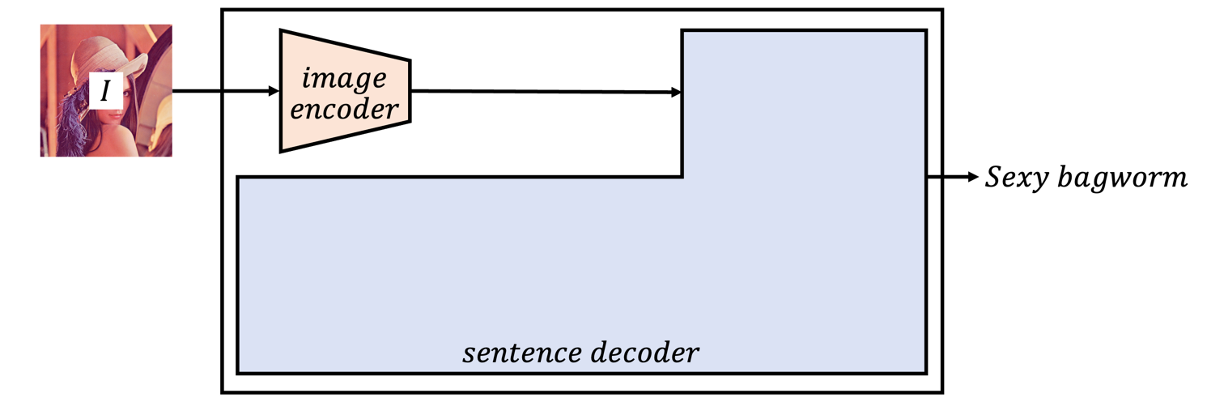
\includegraphics[width=\textwidth]{image_caption_example.png}
    \caption{The data flow of image caption generative model.} \label{fig_image_caption_example}
\end{figure}

\section{GUMI-AE: Generative model of sUitable Meme sentences for Images using AutoEncoder}
~~ In this section, the proposed model of GUMI-AE is introduced.

\subsection{Image Caption Generative Model} 
~~ In an image caption generative model, an image encoder such as Convolutional Neural Network (CNN) \cite{ref_CNN} transforms an input image into its feature as a vector. The feature is used as the conditions for the generation of sentences by the sentence decoder. The structure of the image caption generative model is shown in figure \ref{fig_image_caption}, where $ \bf{I} $ and $ w_t $ denote an input image and the $ t-th $ word of the sentence, respectively. The input image of $ \bf{I} $ is converted into the feature that is typically constructed by a vector. The word $ w_t $ is transformed into embedding the vector and processed by Recurrent Neural Network (RNN) \cite{ref_RNN} such as LSTM \cite{ref_LSTM}. The RNN's internal state $ r_{t} $ at the time step $ t $ is also input and processed considering the time series. Both outputs of the image encoder and RNN are combined and fed into the dense layer. The number of units in this dense layer corresponds to the vocabulary of the image caption generative model, and the output of this layer is converted into a probability distribution via the Softmax function. From the probability distribution produced by the image caption generative model, the $ (t+1)-th $ word of the sentence is either the word with the maximum value or the word selected by the roulette selection, randomly picking a word based on a probability distribution. This procedure is recursively repeated until the token signifying the end of the sentence is selected. 

\begin{figure}[t]
    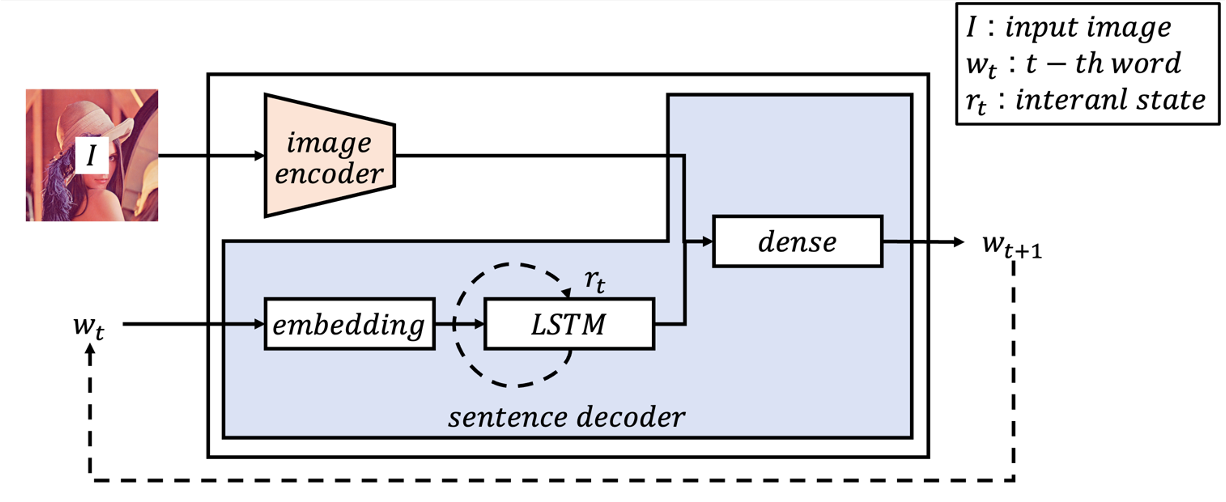
\includegraphics[width=\textwidth]{image_caption_model.png}
    \caption{The structure of the image caption generative model.} \label{fig_image_caption}
\end{figure}

\subsection{AutoEncoder} 
~~ AutoEncoder (AE) is proficient in feature extraction and dimensionality reduction of input data. It consists of an encoder and a decoder and is trained with the objective of (\ref{equation_autoencoder}) reconstructing the input data.

\begin{equation} \label{equation_autoencoder}
    \underset{{\bf p}_e, {\bf p}_d}{\rm min} E(\bf {X}, \it{decoder}(\it{encoder}(\bf X))), 
\end{equation}

\noindent where $ {\bf p}_e $, $ {\bf p}_d $, and $ E $ denote the parameters of the encoder and the decoder and an arbitrary error function such as the mean square error (MSE) respectively, and $ {\bf X} $ is the input to the AE, and $ encoder({\bf X}) $ and $ decoder({\bf X}) $ were the outputs of the encoder and decoder, respectively. Thus, data annotations are not required during the training of AE since the parameters are trained so that the input and the teacher signal of AE are the same. The encoder and decoder can be defined using arbitrary structures, such as CNN \cite{ref_CNN} for images and RNN \cite{ref_RNN} for texts. 

\subsection{GUMI-AE} 
~~ Conventional image caption generative models generating memes for images \cite{ref_Dank_Learning,ref_NJM} typically used a pre-trained image recognition model as the images encoder. However, if this pre-trained model failed to extract image features effectively during the sentence decoder training, it might not generate suitable humorous sentences for the images. One solution to this problem is to retrain the image encoder using the images for the memes, but this approach requires annotations of the images, which many datasets do not have. For example, Bokete \cite{ref_Bokete} images used in the conventional model of NJM \cite{ref_NJM} have no annotations. It is difficult and time-consuming for humans to annotate such datasets. To deal with this problem, this research proposes a new image caption generative model as GUMI-AE that uses the encoder of the AutoEncoder trained with the images of meme dataset in advance as the image encoder of the image caption generative model. \\
~~ The training procedure and structure of the proposed model are shown in figure \ref{fig_proposed} and algorithm \ref{algorithm_GUMI_AE}. Steps 1 through 5 in algorithm 1 train AutoEncoder, and this additional step is different from \cite{ref_Dank_Learning} and \cite{ref_NJM}. Steps 6 through 12 train the image caption generative model as in \cite{ref_Dank_Learning} and \cite{ref_NJM}. In figure \ref{fig_proposed}, the AutoEncoder (AE) is initially trained using images from the dataset. Then, the image caption generative model uses images and sentences from the same dataset. In this process, images are converted into features by passing them through the encoder of the pre-trained AutoEncoder. During the image caption generative model training, the parameters of the pre-trained encoder of AE are frozen and not retrained, thus reducing the number of parameters used and improving training efficiency. In contrast to conventional image caption generative models that use pre-trained models \cite{ref_Dank_Learning} \cite{ref_NJM}, the image encoder in the proposed GUMI-AE is trained using the images of the dataset.

\begin{figure}
    \centering
    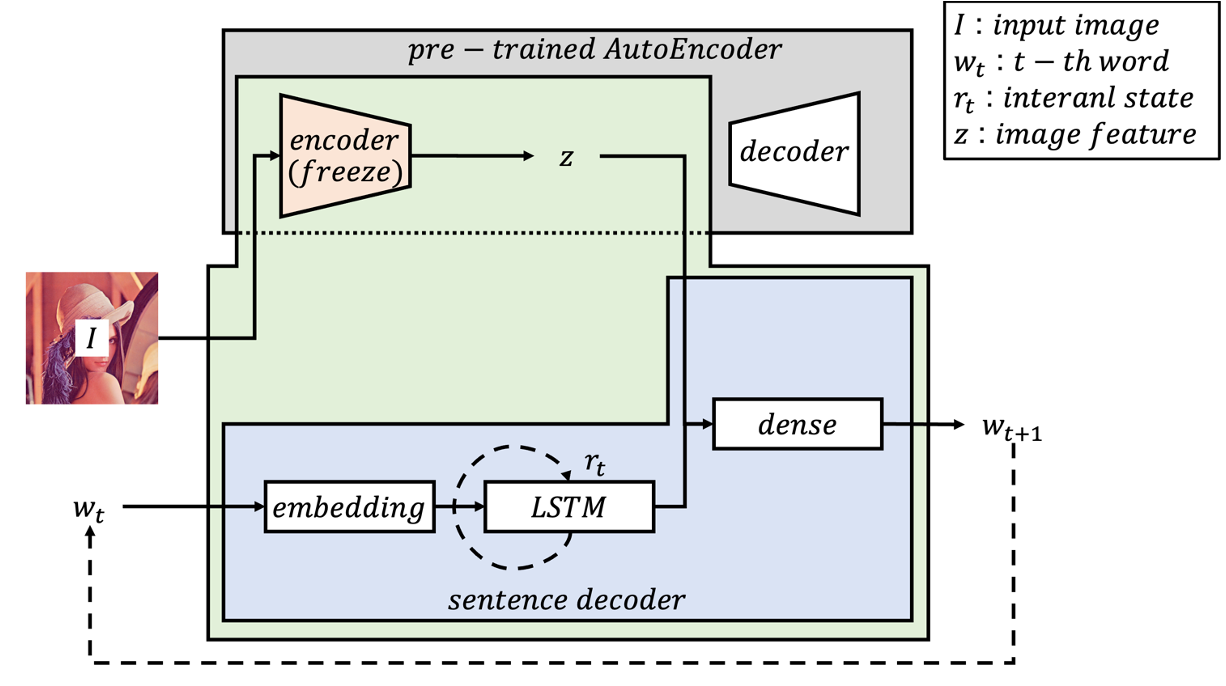
\includegraphics[width=\textwidth]{proposed_method.png}
    \caption{The model structure of the proposed GUMI-AE.} \label{fig_proposed}
\end{figure}

\begin{algorithm}
    \caption{Training procedure of proposed GUMI-AE}
    \begin{algorithmic}[1]
        
        \Require 
            images of meme dataset : $ \mathbf{I} = \{ \mathbf{I}_1, \mathbf{I}_2, ..., \mathbf{I}_N \} $, 
            sentences meme dataset : $ \mathbf{S} = \{ \mathbf{S}_1, \mathbf{S}_2, ..., \mathbf{S}_N \} $,
            parameters of encoder : $ \mathbf{w}_{e} $,
            parameters of decoder : $ \mathbf{w}_{d} $,
            parameters of LSTM : $ \mathbf{w}_{l} $,
            parameters of dense layer : $ \mathbf{w}_{f} $,
            AutoEncoder training epoch : $ k_{a} $,
            image caption model training epoch : $ k_{b} $,
            loss function: $ E $

        % training roop of AutoEncoder
        \For{$ i = 1 $ to $ k_{a} $}
            \State $ \mathbf{z} = encoder_{\mathbf{w}_{e, i}}(\mathbf{I}) $ 
            \State $ \hat{\bf I} = decoder_{\mathbf{w}_{d, i}}(\mathbf{z}) $
            \State update $ \mathbf{w}_{e, i}, \mathbf{w}_{d, i} $ to minimize $ E(\bf{I}, \hat{\bf{I}}) $
        \EndFor
        
        % training roop of image caption model
        \For{$ i = 1 $ to $ k_{b} $}
            \State $ \mathbf{z} = encoder_{\mathbf{w}_{e}}(\mathbf{I}) $
            \State $ \mathbf{y}, \mathbf{r}_i = lstm_{\mathbf{w}_{l, i}}(\mathbf{S}, \mathbf{r}_{i-1}) $
            \State $ \mathbf{x} = Concatenate(\mathbf{z}, \mathbf{y}) $
            \State $ \mathbf{p} = dense_{\mathbf{w}_{f, i}}(\mathbf{x}) $
            \State update $ \mathbf{w}_{l, i}, \mathbf{w}_{f, i} $ to minimize $ E(\bf{S}, p) $
        \EndFor
        
    \end{algorithmic}
    \label{algorithm_GUMI_AE}
\end{algorithm}

\section{Experimental Results}
~~ This section demonstrates the result of the memes for the images generated by GUMI-AE compared with the conventional model of NJM \cite{ref_NJM}. In addition, the details of the training dataset required to generate the memes, the evaluation of the reproducibility of the images by AutoEncoder, and the interestingness of the generated memes will be discussed.

\subsection{Dataset for Training}
~~ Training an image caption generative model to generate memes for images requires a dataset in which images are paired with memes. However, no such dataset currently exists in the available open datasets. In this study, following the approach of \cite{ref_NJM} to create our dataset by scraping the Bokete \cite{ref_Bokete} website which collects images of Japanese memes. The collected dataset consists of 69,365 images with 552,613 Japanese memes. These images were obtained starting with the earliest images posted on the Bokete. There are multiple memes per image. As a preprocessing step, special characters such as "\text{!}" and "\text{?}" from datasets were removed, and eliminated memes containing words that appear less than five times across the entire dataset. The number of memes suitable to a given image varied depending on the image.

\subsection{Training of AutoEncoder}
~~ This section details the training process of AutoEncoder (AE) for the image encoder of the proposed image caption generative model. The architecture of the encoder of AE used here consists of six convolution layers and one dense layer, whose output dimension is 16,384, and the decoder consists of one dense layer and six deconvolution layers. The detailed encoder and decoder construction is shown in figure \ref{autoencoder_construction}. The red, orange, and blue lines indicate convolution, fully connected, and deconvolution. For each convolution and deconvolution layer, the kernel size is 3x3 and the stride is 2. The output of the decoder's output layer is input to the sigmoid function, and the outputs of all other layers are input to the LeakyReLU function. During AE training, each pixel of images is a normalized value ranging from 0 to 1. The MSE was set as the loss function and Adam ($ \eta=0.001,\beta_1=0.999,\beta_2=0.9 $ ) \cite{ref_Adam} as the optimizer. The mini-batch size is 32, and the maximum training iterations is 150. Table \ref{table_result_AutoEncoder} shows the training results of the AE. The input images in Table \ref{table_result_AutoEncoder} were not used during training. The training results suggest that the implemented AE can adequately reconstruct the input image. This indicates that the AE encoder effectively extracts the image features.

\begin{figure}[t]
    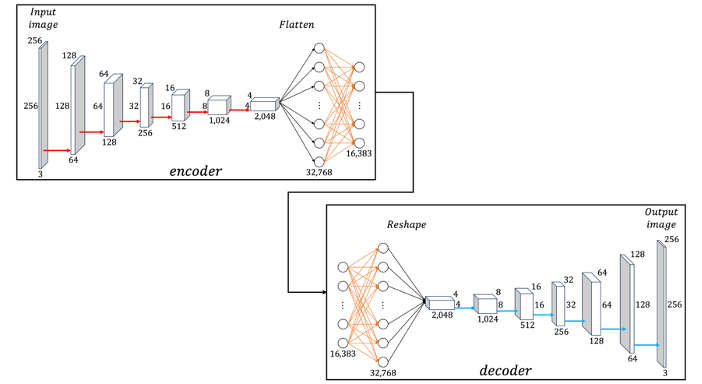
\includegraphics[width=\textwidth]{autoencoder_construction.png}
    \caption{The construction of AutoEncoder.} \label{autoencoder_construction}
\end{figure}

\begin{table}[t]
  \centering
  \caption{The training result of AutoEncoder}
  \begin{tabular}{|c|c||c|c|} 
    \hline
        input & output & input & output \\
    \hline

    \hline
        \begin{minipage}{0.24\textwidth}
            \centering
            \scalebox{0.25}{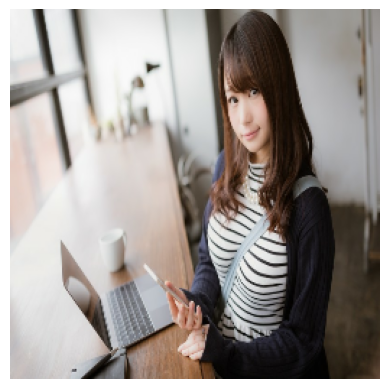
\includegraphics{autoencoder_input_1.png}}
        \end{minipage} &
    
        \begin{minipage}{0.24\textwidth}
            \centering
            \scalebox{0.25}{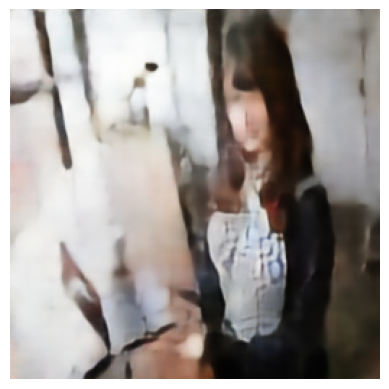
\includegraphics{autoencoder_output_1.png}}
        \end{minipage} &

        \begin{minipage}{0.24\textwidth}
            \centering
            \scalebox{0.25}{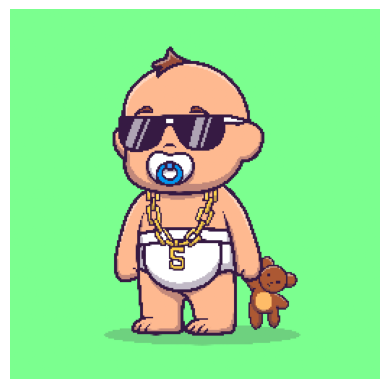
\includegraphics{autoencoder_input_2.png}}
        \end{minipage} &
    
        \begin{minipage}{0.24\textwidth}
            \centering
            \scalebox{0.25}{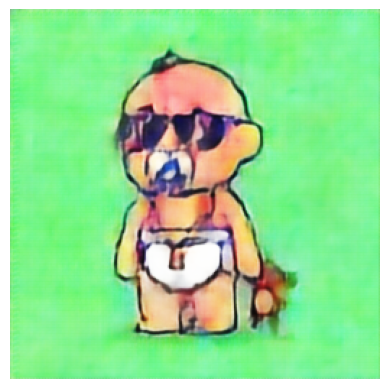
\includegraphics{autoencoder_output_2.png}}
        \end{minipage} \\ 
    \hline
    
  \end{tabular}
  \label{table_result_AutoEncoder}
\end{table}

\begin{figure}[b]

    \centering
    \begin{minipage}[t]{0.49\textwidth}
        \centering
        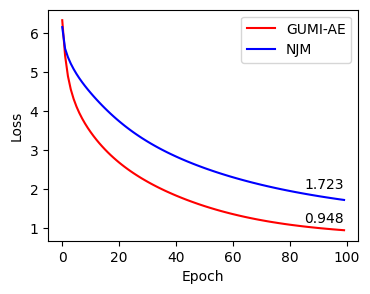
\includegraphics[width=\linewidth]{train_loss.png}
        \caption{Train loss per epochs.}
        \label{fig_train_loss}
    \end{minipage}
    % \hspace{0.5cm} % 画像の間にスペースを追加する
    \begin{minipage}[t]{0.49\textwidth}
        \centering
        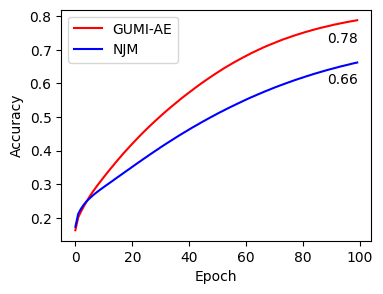
\includegraphics[width=\linewidth]{train_accuracy.png}
        \caption{Train accuracy per epochs.}
        \label{fig_train_accuracy}
    \end{minipage}
    
\end{figure}

\subsection{Training of Meme Generator}
~~ To investigate the effectiveness of the proposed method GUMI-AE, two models are implemented to generate memes for images. The first model is the conventional NJM \cite{ref_NJM}, which uses ResNet152 pre-trained on ImageNet \cite{ref_NJM,ref_ResNet152,ref_ImageNet} as the image encoder, and the second is the proposed GUMI-AE. In this experiment, NJM and GUMI-AE are trained on the same dataset introduced in subsection 3.1. The structures of sentence decoders in both models are 1,024 LSTM units, 2 total dense layers, 2,048 hidden layer units, and 48,480 output layer units, respectively. The loss function is categorical cross-entropy, and the optimizer is Adam ($ \eta = 0.001, \beta_1 = 0.999, \beta_2 = 0.9 $ ) \cite{ref_Adam}. The mini-batch size was set to 2,048 and the maximum number of training epochs was set to 100. The input images are standardized to a resolution of 224 pixels each in height and width because of the input size of the pre-trained ResNet152. \\
~~ The results are shown in figures \ref{fig_train_loss} and \ref{fig_train_accuracy} which show the training loss per epoch and the training accuracy per epoch, respectively. In both figures, the proposed model GUMI-AE is drawn in red and the conventional model NJM is drawn in blue. These figures show that the proposed method has low training loss and high training accuracy. Therefore, it is concluded that GUMI-AE has better model performance. Since the two image caption generative models differ only in the image encoder and have the same network structure. The proposed structure namely, using AutoEncoder as a sentence decoder is suitable for the training performance of the image caption generative model.\\
~~ Next, four sample memes generated by GUMI-AE and NJM and their input images are shown in Table \ref{table_generated_memes}. These images are not used in the training process. Each meme word is chosen by the roulette selection, which randomly selects a word according to a probability distribution output by an image caption generative model. This allows multiple sentences to be generated for a single image. Table \ref{table_generated_memes}(a) is the result of the illustration of Japanese Kabuki input. For this image, GUMI-AE generates the meme "Where's Wally". This meme is thought to be generated because the character in the illustration is similar in color scheme to the character in the picture book "Where's Wally?". It also can be seen that the Meme generated by NJM contains words that have no possible relevance to the image, such as "pot" and "tadpole". Table \ref{table_generated_memes}(b) is the result of the illustration of the baby wearing only the diaper input, and GUMI-AE generates the meme "Your zipper is open" for this image. Commenting "Your zipper is open" on the baby's diaper can cause a kind of misunderstanding or confusion since diapers usually do not have zippers. This creates a humorous surprise, an unexpected reversal, and a laugh. Contrary to this, the meme generated by NJM contains the unrelated word "sea". These two results show that GUMI-AE is able to extract features from illustration images more accurately than NJM. 
Table \ref{table_generated_memes}(c) is the result of inputting the photo of the woman. NJM fails to generate a meme that contains words that are relevant to the image, despite GUMI-AE generating a meme containing the word "Mam" and related words. This may be due to the fact that NJM's feature extractor is not highly accurate. Table \ref{table_generated_memes}(d) is the result of inputting the image contained in ImageNet. In response to the image of a starfish posing on land, GUMI-AE generates the sentence "Perform one last gag," which is a funny meme as it shows that the starfish is no longer able to move after being on land.NJM generated the meme "Captured jellyfish," which is also funny because it mistakes a starfish for a jellyfish. From these results, the proposed model GUMI-AE can generate more suitable memes for an image than NJM because of its higher learning accuracy, but it is considered that NJM can also generate suitable memes for the same image that has been pre-trained.

\begin{table}[!t]
    \caption{
        The memes generated by GUMI-AE and NJM.
    } 
    \centering
    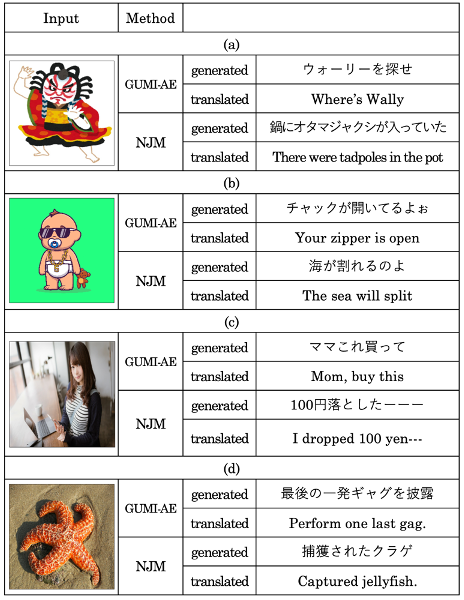
\includegraphics[width=\textwidth]{generated_memes.png}
    \label{table_generated_memes}
    
\end{table}

\begin{figure}[t]
    \centering
    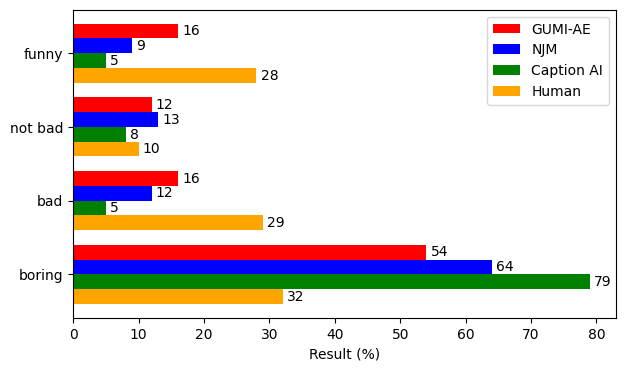
\includegraphics[width=10cm]{questionnaire_result.png}
    \caption{
        The questionnaire results.
    } 
    \label{fig_questionnaire_result}
\end{figure}

\subsection{Evaluation of humorous}
~~ Next, evaluating the proposed and conventional methods concerning humor ability is discussed. Unfortunately, at the present stage, it is impossible to automatically assess the humor ability of the generated memes. Therefore, in this study, as in the conventional NJM \cite{ref_NJM} method, the humor ability of the sentences is evaluated by a questionnaire. The number of responding questionnaires was 509. As the target of the questionnaire, the sentences created by humans and uploaded in Bokete \cite{ref_Bokete}, and the sentences generated by the proposed method GUMI-AE, NJM \cite{ref_NJM}, and image caption generative model which uses a pre-trained model trained with STAIR caption dataset \cite{ref_STAIR_Caption}, the conventional research used \cite{ref_NJM}. As a questionnaire environment, one input image and one meme of each method were randomly selected and were shown on BoT which was created on one of the most particular SNS in Japan named LINE \cite{ref_LINE}. Respondents were allowed to look at the displayed image and meme and comment on them in four levels: "funny", "not bad", "bad" and "boring". Note that respondents only know whether the memes relative to the images are funny or not. The results of the questionnaire survey are shown in figure \ref{fig_questionnaire_result}. In figure \ref{fig_questionnaire_result}, the vertical axis is a four-level rating, and the horizontal axis is the percentage of responses. In the graph, red indicates the proposed method GUMI-AE, blue indicates NJM, green indicates caption AI, and orange indicates human. In this paper, the results "funny" and "not bad" are considered positive responses, and the items "bad" and "boring" are considered negative responses. Figure \ref{fig_questionnaire_result} shows that the caption AI trained on the STAIR Caption dataset receives more negative responses than the AI trained on the dataset combining images and memes. On the other hand, the proposed method GUMI-AE receives a 6\% higher positive evaluation than the conventional method NJM. This is likely due to the higher suitability of the image encoder of the image caption generative model of the proposed method and the more accurate training of image captioning with the images in the training dataset. Comparing the proposed method GUMI-AE with humans, the percentage of positive responses to human memes is higher. One of the reasons for this result can be attributed to the fact that the proposed method uses roulette selection to select words from the probability distribution generated by the model, which sometimes results in the selection of inappropriate words. Therefore, it can be concluded that the proposed method GUMI-AE, even though it is inferior to the humor of human memes, is more accurate than the conventional model using pre-trained models for the image encoder of image caption generative model, and can generate memes that are appropriate for the images.

\section{Conclusion}
~~ This paper proposed a new model, GUMI-AE, which uses the encoder of the AutoEncoder as the image encoder of the image caption generative model to generate memes appropriate for the Japanese meme "Ohgiri" for the images. Conventionally, an image caption generative model with pre-trained models as the image encoder has been used as an AI to generate memes for images. However, when using the pre-trained model, if there is domain divergence between the images for pre-training and the images for image caption training, the feature of the input image is not correctly extracted, and the meme suitable for the image cannot be created. To deal with this problem, a new model GUMI-AE, which uses the encoder of the AutoEncoder instead of pre-trained models was proposed in this paper. Experimental results show that the proposed model has higher learning accuracy than the conventional model and successfully generates memes suitable for images. In addition, since the encoder of AutoEncoder is used, the network structure can be freely configured, which has the advantage of matching the computational resources. \\
~~ In future research, we will implement a generator using advanced networks such as Gated Recurrent Unit and Transformer to generate memes with higher accuracy and investigate the impact of the questionnaire on the results by taking into account the age and gender of the participants.

\subsubsection{Acknowledgements}
This work is supported by The Japan Society Promotion of Science
(JSPS), KAKENHI (23K11267).


\begin{thebibliography}{18}

\bibitem{ref_GAN}
Goodfellow, I., and et al.: Generative adversarial networks. {\it Communications of the ACM}, 63(11), 139-144 (2020).

\bibitem{ref_ChatGPT}
OpenAI, https://chat.openai.com, ChatGPT. Last Accessed 6 June 2023

\bibitem{ref_Show_And_Tell}
Vinyals, O., and et al.: Show and tell: A neural image caption generator. {\it Proc. IEEE Computer Vision and Pattern Recognition (CVPR)}, pp. 3156-3164 (2015).

\bibitem{ref_meme}
Akhther, N.: Internet Memes as Form of Cultural Discourse: A Rhetorical Analysis on Facebook. {\it PsyArXiv} (2021).

\bibitem{ref_ResNet152}
He, K., Zhang, and et al.: Deep residual learning for image recognition. {\it Proc. IEEE Computer Vision and Pattern Recognition (CVPR)}, pp. 770-778 (2016).

\bibitem{ref_Inception_v3}
Szegedy, C., and et al.: Rethinking the inception architecture for computer vision. {\it Proc. IEEE Computer Vision and Pattern Recognition (CVPR)}, pp. 2818-2826 (2016).

\bibitem{ref_ImageNet}
Deng, J., and et al.: Imagenet: A large-scale hierarchical image database. {\it Proc. IEEE Computer Vision and Pattern Recognition (CVPR)}, pp. 248-255 (2009).

\bibitem{ref_Dank_Learning}
Peirson, V., and et al.: Dank learning: Generating memes using deep neural networks. arXiv preprint arXiv:1806.04510 (2018).

\bibitem{ref_NJM}
Yoshida, K., and et al.: Neural joking machine: Humorous image captioning. {\it Proc. IEEE Computer Vision and Pattern Recognition Conference (CVPR) Language and Vision workshop} (2018).

\bibitem{ref_Memegenerator}
Memegenerator.net, https://memegenerator.net. Last Accessed 7 June 2023

\bibitem{ref_Bokete}
Omoroki INC., https://bokete.jp, Bokete. Last Accessed 7 June 2023

\bibitem{ref_AutoEncoder}
Hinton, G. E., and et al.: Reducing the dimensionality of data with neural networks. {\it science}, 313(5786), 504-507 (2006).

\bibitem{ref_LSTM}
Graves, A., and et al.: Long short-term memory. {\it Supervised sequence labeling with recurrent neural networks}, 385, Springer, pp. 37-45 (2012).

\bibitem{ref_CNN}
LeCun, Y., and et al.: Gradient-based learning applied to document recognition. {\it Proceeding of the IEEE}, 86(11), 2278-2324 (1998).

\bibitem{ref_RNN}
Williams, R. J., and et al.: A learning algorithm for continually running fully recurrent neural networks. {\it Neural Computation}, 1(2), 270-280 (1989).

\bibitem{ref_Adam}
Kingma, D. P., and et al.: Adam: A method for stochastic optimization. {\it Proc. International Conference on Learning Representations (ICLR)}, pp. 1–13 (2015).

\bibitem{ref_STAIR_Caption}
Yoshikawa, Y., and et al.: STAIR Captions: Constructing a Large-Scale Japanese Image Caption Dataset, {\it Proc. Annual Meeting of the Association for Computational Linguistics (ACL)}, 2, pp. 417–421 (2017).

\bibitem{ref_LINE}
LINE Corp., https://linecorp.com, LINE. Last Accessed 7 June 2023

\end{thebibliography}
\end{document}